\documentclass[11pt, oneside]{article}   	% use "amsart" instead of "article" for AMSLaTeX format
\usepackage{geometry}                		% See geometry.pdf to learn the layout options. There are lots.

\geometry{letterpaper}                   		% ... or a4paper or a5paper or ... 
%\geometry{landscape}                		% Activate for rotated page geometry
\usepackage[parfill]{parskip}    			% Activate to begin paragraphs with an empty line rather than an indent
\usepackage{graphicx}				% Use pdf, png, jpg, or eps§ with pdflatex; use eps in DVI mode
								% TeX will automatically convert eps --> pdf in pdflatex
\usepackage{amssymb}

\usepackage{hyperref} 				% you need this package
\usepackage{pifont}					% for \ding

% Make clickable footnote
\newcommand{\hyperfootnote}[1][]{\def\ArgI{{#1}}\hyperfootnoteRelay}
  % relay to new command to make extra optional command possible
\newcommand\hyperfootnoteRelay[2][]{\href{#1#2}{\ArgI}\footnote{\href{#1#2}{#2}}}
  % the first optional argument is now in \ArgI, the second is in #1
  
% Takes at most 3 parameters (see http://www.tex.ac.uk/FAQ-twooptarg.html for info on multiple optional parameters)
% If first parameter isn't given, it's value is '' (empty string in text before footnote reference)
% If second parameter isn't given, it's value is '' (string before visible URL, e.g. 'http://')
% Makes a clickable footnote (alternatively: \url{}) with optional reference in the text as well
% Use 1: \hyperfootnote{www.mywebsite.com}: creates a footnote consisting of a clickable URL
% Use 2: \hyperfootnote[My website]{www.mywebsite.com}: creates a clickable piece of text in the text ('My website') plus a footnote consisting of a clickable URL
% Note: requires the hyperref package.
% Note: use xspace package to add/absorb spaces when necessary (e.g. to avoid a space between the footnote number and a punctuation mark)

% Info on how to define a LaTeX command: https://www.sharelatex.com/learn/Commands

%SetFonts

\title{Identity Agents}
\author{Paul Trevithick, The Mee Foundation}
%\date{}							% Activate to display a given date or no date

\begin{document}
\maketitle

\section{Power Asymmetry}
While the internet has brought new services and experience to billions of users, it has also resulted in a power asymmetry between the digital service providers and their users regarding these users' digital identities and personal data. These providers have accumulated power relative to their users.

The internet's designers endeavored to create decentralized architectures that pushed computation and storage to the edge and minimize centralized control. However, in the last couple decades economic factors and so-called natural monopolies, preferential attachment network effects, economies of scale, and the relative ease of creating centralized solutions have all contributed to concentrations of power on the provider side. 

When Berners-Lee created the web, it was a decentralized platform. Anyone could publish a website and link to any other side. But as the web has grown from an obscure research-sharing community into a global medium for commerce, communication, journalism and entertainment, the power dynamics have shifted. Today, huge companies like Amazon, Meta, Google, and Netflix dominate the web. These corporate giants enjoy an enormous amount of control not only over what people see and do online but over users' private data.\cite{Finley2017}

In response, many initiatives and projects are propose alternative approaches and technologies. Here are just a few examples: \hyperfootnote[rececentralize.org][https://]{redecentralize.org}, \hyperfootnote[DWeb principles][https://]{getdweb.net/principles/}, \hyperfootnote[The Web3 Foundation][https://]{web3.foundation/}, \hyperfootnote[the Decentralized Identity Foundation(DIF)][https://]{identity.foundation}, \hyperfootnote[``local-first" software principles][https://]{inkandswitch.com/local-first/}, \hyperfootnote[ProjectVRM][https://]{blogs.harvard.edu/vrm}, \hyperfootnote[Blue Sky][https://]{blueskyweb.xyz/}, and the \hyperfootnote[Decentralized Information Group][https://]{dig.csail.mit.edu}. 

To reinforce our focus on power relationships, we use the term \emph{computational power} to refer to software tools that work (i.e. provide agency) ``on the user's side" for, and \emph{exclusively} on behalf of, the user. We are not talking about whether the average user's phones and laptops have sufficient computational power; they do. We're saying that this raw computational power and storage is not leveraged by tools that push back on app provider's power, and engage digitally and automatically to empower the user to better manage their relationships with providers on terms more beneficial to them. Since our discussion applies equally provider's mobile apps, webapps, and websites, we simply use the term \emph{app} to refer to all of them.

Power asymmetry lies at the root of a diverse set of related symptoms, most of which erode privacy, since privacy and power are highly interrelated concepts\footnote{Consider the title of V\'eliz's recent book, ``Privacy is Power"\cite{veliz2020}}. 
These privacy eroding symptoms include a lack of personal autonomy, a lack of personal agency, and third-party surveillance. 

\subsection{Lack of Autonomy}

\begin{quote}
\textbf{au\hspace{0.5mm}\tiny \ding{108}\normalsize \hspace{0.5mm}ton\hspace{0.5mm}\tiny \ding{108}\normalsize \hspace{0.5mm}o\hspace{0.5mm}\tiny \ding{108}\normalsize \hspace{0.5mm}my}: \emph{freedom from external control or influence; independence.}\hyperfootnote[][https://]{languages.oup.com/google-dictionary-en/}
\end{quote}

\emph{Independence}. In the physical world each of us is a separate, independent entity. Each of us has a self that embodies our individuality. We ``bring" that independent selfness to interactions with others, with vendors, etc. while understanding that this independence is not absolute--we are still to some extent dependent on common, shared systems, laws, environments, and so on. By contrast, online it has been said that ``we have no \emph{digital embodiment}."\footnote{Phil Windley, personal communication, Sepember 2022}  Our identities are provided to us by digital service providers (e.g. in the form of a Facebook identity, or an Amazon account). Without them we don't exist. Anyone who has been banned from a platform, or uses a platform that is shut down is sharply reminded that their digital identity exists at the pleasure of that platform. Our provisional existence is the original power asymmetry. Efforts create personal datastores, or even more to the point, those that strive to provide each of us a \emph{self-sovereign identity}\cite{Preukschat2021} are squarely aimed at addressing this issue--the word ``sovereignty" certainly evokes power.

\emph{Ownership}. Our personal data is collected and held by businesses (first-parties) as we interact with their apps, not by us. This pattern \emph{app-held data} is so common that it's hard to imagine an alternative. Our data is not free from external control by apps, because it is generally stored and managed by them. 

Our data is also collected and held by third-parties (e.g. data brokers) with whom we have no interactions at all. In short, it's been said that \hyperfootnote[“everybody has our data … except us.”][https://]{reb00ted.org/personaldata/20210620-who-has-my-personal-data/}. 

As we'll discuss more later on, there are alternative approaches. One is ``user-held" data\cite{Jurcys2021}, where your data is held by you in a personal datastore)\footnote{Examples of open-source personal datastores include \url{https://solidproject.org}, Decentralized Web Nodes(DWN). For more about personal datastores see \url{https://wikipedia.org/wiki/Personal\_data\_service}}. Another is following ``local-first" software principles.\cite{Kleppmann2019}

\emph{Lock-in}. As we've just mentioned our online existence is provisional. Further, this existence is bound to the provider from which it originated. Providers hold our data, and although in many jurisdictions providers are required to allow us to have access (e.g. to request that we can download a copy), we lack the technical means to accept the data stream and hold (e.g. in a personal datastore) that has the ability to subsequently transform it into other formats and schemas so as to make it reusable in other contexts. This lack of agency results in our data being held hostage, i.e. without autonomy. 

\emph{Peer-to-peer} With a few exceptions, e.g. technologies like Berty\hyperfootnote[][https://]{berty.tech}, internet users, when they communicate person-to-person don't have the ability to do so \emph{peer-to-peer} from their edge devices to the other person's device. Instead, they are dependent on servers hosted by intermediaries. Whereas these days the messages themselves are end-to-end encrypted, the metadata (e.g. who a person communicates with, from where, at what time, how often and from which device, etc.) is in many cases visible to the intermediary's server. 

\subsection{Lack of agency}

\begin{quote}
\textbf{a\hspace{0.5mm}\tiny \ding{108}\normalsize \hspace{0.5mm}gen \tiny \ding{108} \normalsize cy}: \emph{the capacity, condition, or state of acting or of exerting power} \hyperfootnote[][https://]{www.merriam-webster.com/dictionary/agency}
\end{quote}

\emph{Wielding credentials}. In the offline world you can autonomously present your drivers license to a wine seller in order to prove that you are of drinking age since the wine seller trusts the license issuer. The interaction is privacy-respecting because the presentation interaction is not disclosed to the issuer. This could be described as ``wielding" a trust credential. At present, there is no equivalent way to do this online. There's no standard way to be issued a credential, hold that credential in digital wallet, and then present that credential. With a few, domain-specific exceptions (e.g. cryptocurrency), there is no common, generalized method for you to prove something about yourself as stated by one party about you, to another party online.

\emph{Data presentation}. One reason for form filling and other kinds of data entry on providers apps/sites is that the user, even if they were equipped with a personal datastore, lacks the ability to present personal information digitally to the provider. Instead the information must be re-entered manually at each provider. The credential presentation interaction mentioned above provides specialized example.

\emph{Delegation}. In the offline world one entity can grant access to some resource to another entity. For example, I could give my car keys to a friend so they could borrow my car. There is no standard, or secure way to do this online. This is especially problematic in healthcare scenarios where a caregiver needs to gain access to electronic health-related data about another person.

\emph{Provider-defined Privacy Policies}. Users are given the option to review the privacy policies put forth by the provider, policies which are designed to protect the provider's interests while staying within the limits defined by the relevant privacy regulations. The burden of making sense of these policies is shifted to the user (i.e. the potential victim) because the user doesn't have the time to read 100+ policies for the providers they typically use, nor do they have the computational power on their side to aid them in this assessment. 

\emph{Privacy policy expression}. With a few exceptions, (e.g. the \hyperfootnote[Global Privacy Control][https://]{globalprivacycontrol.org}), users  lack the technical means (i.e. computational power) to express their privacy terms to providers. 

\emph{User rights}. In a growing number of jurisdictions, starting with Europe's GDPR and expanding to other regions, the user's data rights, (e.g. the right to access, correct and delete their data), are explicitly stated. In principle these laws respect these rights, however in practice the time and effort required to exercise these rights is so exorbitant, that in practice they don't exist. The user has to send written requests to get their data, request that it by updated or deleted, etc. User-side agents are required for user's to regain in practice the rights they have in principle. 

\emph{Inferences}. "Eli Pariser need to give users control of their bubble" check this quote\cite[p66]{McNamee2020}(interests profile)

\emph{Feudalism}. [You (as a peasant) work the fields, the landlord owns them and amass fortunes; mentions of Jared's and others AI injustice about who owns the work. Jared Lanier, etc.]

\subsection{Third-party surveillance}

Whereas the user is at least aware when they sign up on a first-party app that their interactions are known to the provider of that app, there are hundreds of third-parties of which the user is unaware that track and assemble databases about them. Databases of user data in the hands of hundreds of unknown third-parties creates privacy risks and vulnerabilities. Users have little transparency into what's being gathered, where it's being shared and how it's being used. It is worth noting that that much of this third-party tracking is enabled in collaboration with first-parties (e.g. first-parties placing third-party tracking cookies on the user's browser).

\emph{Surveillance-based targeted advertising}. Targeted advertising in general\footnote{Also known as behavioral advertising or more recently, interest-based advertising} involves four main processing steps: (1) the collection of observations about the user by a first- or third-party, (2) synthesis of an "ad profile” from these observations, (3) matching this ad profile against available "target audiences”(i.e. characteristics of whom the advertiser wishes to reach, advertising budget, etc.) from advertisers through a bidding process, and (4) displaying the winning ad. Surveillance-based targeted advertising specifically is when step (1) above is achieved by third-parties who track the user as they move from apps to app and site to site across the internet using third-party cookies and similar tracking mechanisms. 

Third-party ad tech vendors perform the tracking and synthesis of a user's "ad profile." Users have no say in their own ad profiles--never seeing them and not the ability to correct them.

\emph{Data brokers}. Data brokers who buy and sell personal data to other brokers, to advertisers, adtech firms and first-party publishers provide liquidity (along with a host of privacy threats) in the personal data shadow marketplace because user's lack the computational power to provide data about themselves.

\subsection{Inconvenience}
The prevailing architecture of the internet involves each provider managing their own  information ``silo" of information about the user (i.e. their account). This approach and the lack of computational power on the user's side creates inconvenience for them that is described below.

\emph{Repetition}. When using apps, users ")are often asked to provide information about themselves that another app has already asked them such as ``what is your email address?" This is a symptom of the internet's silo-ed architecture wherein each app maintains its own database of personal information. The user has the hassle of repeated data entry, the app has increased friction (a worsened user experience).

\emph{Password management}. The average user uses 100 websites and 25 apps daily. Managing and periodically updating strong, unique passwords at each is  impractical without an automated password manager (computational power), yet it has been estimated that less than 5 percent of internet users use a password manager. 

\emph{Account Management}. The user has the inconvenient burden of maintaining the timeliness and consistency of their account information at over one hundred apps. For example, updating contact or credit card information at each is tedious, time-consuming and encourages the user to spend more time at sites that already have their information. The relative convenience of shopping on Amazon vs. another e-commerce site. It is partially caused by the user's lack of computational power to manage these relationships--the processes are not automated and tedious.

\section{Design Considerations}
Our vision is to develop an identity agent to address the problems outlined in the previous section. This agent  can represent the user and promote their interests online. In this section, we discuss a number of design considerations for this agent illustrating the each with use cases.

\subsection{User-centric vs. provider-centric}

Many of the challenges described thus far have their origin in an architecture that is \emph{provider-centric} rather than \emph{user-centric}, or \emph{human-centered}. In the provider-centric model each provider sees a single narrow slice of the user through the lens of their direct interactions with them. Each works in isolation to optimize the user's experience on their app or at their site. To the user the situation is reversed. They sit at the center of many dozens of connections radiating out from them to apps/sites. The user has the burden for entering, and updating information at each provider each of which maintains a separate copy. 

The best technology so far to address this user burden is a browser form-fillers which greatly reduces the number of keystrokes required to fill in web forms. Browsers are \emph{user-agents} that perform this operation on the user's behalf, and sit on the user's side of the power equation. Another closely related user-agent technology is that of password managers. In both cases these agents maintain small databases on the user's side.

\subsection{Edge-centered vs. cloud-centered}
Given that we need a per-user, user-centric decentralized architecture, where should this datastore live? We look at two options edge-centered and cloud-centered. Edge-centered means that the primary location for a user's personal datastore is on their own phones, and laptops and perhaps home servers. Cloud-centered means that the user's personal datastore is primarily held in the cloud (e.g. on a \hyperfootnote[SOLID][https://]{solidproject.org} pod). We say \emph{primary} because there are usually use-cases that involved replicating/syncing some of the data to the "other" location. 

\emph{Security}. Although some may disagree, it is our contention that having a personal datastore on a personal device is more secure than in the cloud. Even if each platform alternative where equivalently secure, a cloud-centered architecture aggregates millions of personal datastores at one service provider and thereby creates millions of times the economic incentive for hackers to invest in attacking it. 

\emph{Equity}. The hosting costs of a cloud-centered solution must be paid for by some entity whereas user's typically own their edge devices and they are thus on a marginal basis "free". By equity we mean here that we need a solution that can be afforded by all socio-economic classes, and a solution that requires monthly hosting fees can thereby be ruled out. 

\emph{Backup}. One serious drawback of what's called a \emph{non-custodial} edge-centered architecture (when compared to cloud-centered) is the need for the user's data to be backed up. This is not a problem if the user backs up their devices (e.g. to a cloud backup service), but many can't be relied on to be disciplined about this. [stats on phone vs. laptop backup]. [we assume the user has N>1 device and that the agent is installed on N>1 and that the agents replicate/sync]

\subsection{Replication}

If we assume an edge-centered design, we must solve the roaming problem. That is, we must support use cases where the user has more than one device and needs to be able to pick any one of them and have their person datastore be consistent across these devices (at least eventually). This requires that the agents of a given user implement replication and syncing. [discuss the (unfortunate and costly) need for relays to achieve P2P sync in some use cases].

\subsection{Loyalty}

Much of the power asymmetry described in the first section is due to economic incentives for providers to do just enough in the user's interest to keep them as a user or customer, but not more. Personal data, after all, is considered by business to be an asset class; the more of it that is collected and monetized the better. To have an agent that works not partially but exclusively on behalf of the user, the agent provider must not have an economic incentive to provide anything less but complete loyalty to the user's interests. Although there are other potential solutions (e.g. data cooperatives and data unions) we think the simplest approach is that the agent developer be a nonprofit organization that has no economic incentive to be anything but loyal to the user and to have no economic interest in their data. In fact there's no reason that that the agent developer to access or store the user's data.

\subsection{Separation of app from db}

[Talk about this from the point of view of the SOLID project or go-peer?? or ??. Also talk about how this is inevitable. Desktop OSes had it, then in 2007?? iPhone got it, now in 2023! webapps will get it. Talk about automatic data portability]

\subsection{Delegation}

[Talk about delegated medical records use case]. [Talk about the Gropper Principle]

\subsection{Multi-contextual}

Zuckerberg has said "Having two identities for yourself is an example of a lack of integrity"\cite{Kirkpatrick2011}. He could not be more wrong. Let's take a step back and look at selfness and whoness. 

\subsubsection{Selfness and Whoness}

In his \hyperfootnote[last public speech][https://]{www.youtube.com/watch?v=9DExNTY3QAk}  
\hyperfootnote[Kim Cameron][https://]{en.wikipedia.org/wiki/Kim\_Cameron\_(computer\_scientist)} introduced two useful definitions based on archaic English:

\begin{itemize}
\item \textbf{Selfness}: The sameness of a person or thing at all times or in all circumstances. The condition of being a single individual. The fact that a person or thing is itself and not something else. Individuality, personality. 
\item \textbf{Whoness}: Who or what a person or thing is. A distinct impression of a single person or thing presented to or perceived by others. A set of characteristics or a description that distinguishes a person or thing from others. 
\end{itemize}

The following diagram illustrates these concepts and introduces the notion of context:

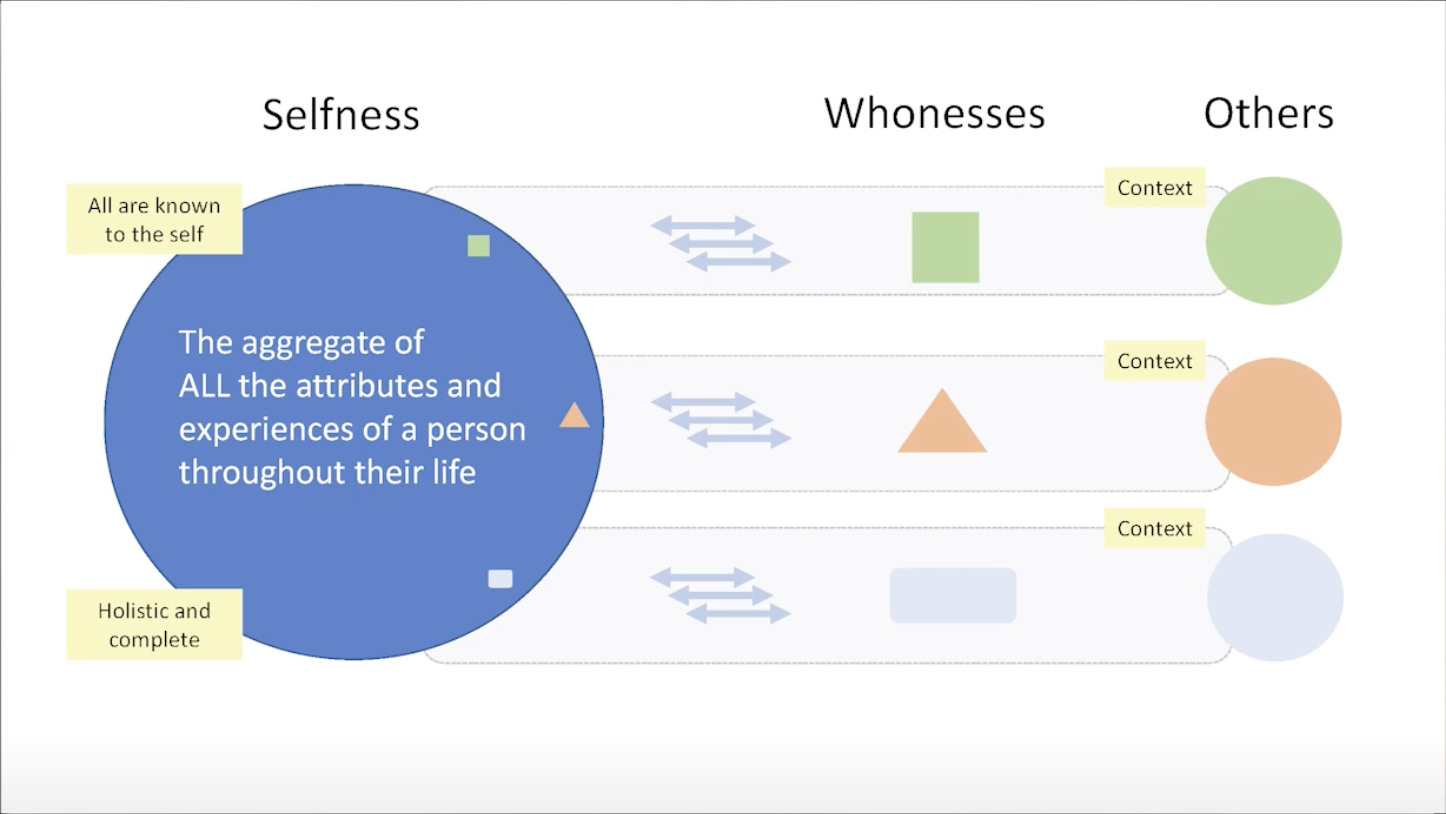
\includegraphics[width=\textwidth]{./images/selfness-and-whoness-larger.png}

\subsection{Open source}

In order to trust that the agent does what we claim, we need transparency which open source can provide. Further this is an ambitious project and we need to nurture the creation of a community of developers help build it.

\subsection{Data Governance}

Once data is shared from the agent to a first-party there are no technical means to constraint what the recipient does with it. No technical means can prevent them from selling it others, for example. Instead, legal means must be employed. Rather than wait for privacy regulations to get strong enough, we propose that first-parties sign a Human Information License to license the user's information under terms that are fair and balanced and respect the user's privacy rights. The contract can be signed by an entity that represents the user to make it effortless for the user.

\subsection{User rights}

[to be written: even the best privacy legislation is impotent in practice to protect users because they don't require associated technical means to implement them]

\subsection{Enforcement}

[to-be-written: Talk here about the need for an entity to audit and enforce compliance with the legal contract]

\subsection{Privacy by design}
[to-be-written]

\section{Identity Agents} %SECTION

\subsection{End-user perspective}
An \emph{identity agent} is an app that gives the user control (power) over their own personal information as they interact with websites, mobile apps, and other user's agents. It does this through a combination of technical and legal mechanisms.

\subsubsection{Privacy and Autonomy} 
The agent runs on the user's edge devices (mobile phone, laptop, etc.) where, entirely under the user's control, it holds a local, private database of the user's personal information. When an app/site wants to know something about the user, the agent shares as much or as little as the user chooses. If an app/site signs a Human Information License and thereby becomes \emph{certified}, the legal entity behind that app/site is thereby obligated to (i) require explicit consent for collection, processing, storage and sharing of the users data and to (ii) implement APIs to exercise the user's rights to access, correct and delete the user's personal information. We envision that agents could provide ad profiles to certified publisher websites that are supported by interest-based advertising while eliminating the need for surveillance by third-parties.

\subsubsection{Convenience}
Although the agent is an interactive application, it operates in the background most of the time. Always working solely in the user's interest, it collects information from sites that already hold their data, and shares it with other sites that need it. Our vision is that that the user *never has to repeat themself* (nor remember passwords!) as they move from app to app and site to site across the internet.

Here are a few examples. If a site wanted to know the user's email address it might ask for it in a web form. In this case the agent would use it's form-filler ``protocol" to fill in the value. If the site supports password-less sign-in (e.g. using OpenID Connect) the agent acts as the identity provider. If a site needed a digital driver's license credential, the agent acts as a digital wallet and presents this credential that it had presumably downloaded earlier from an issuing site. In these different examples, different protocols for information sharing are required, and in the interest of convenience, the agent should support all of them.

\subsection{Self and contexts}
The agent represents both the user's \emph{selfness} and \emph{whonesses}.

The selfness of the user is held in a data container called the \emph{self}. The contents of the self are holistic and therefore quite sensitive. For this reason they would normally not be shared in a direct or comprehensive form with others. The user's self is the point of integration across contexts each of which may be from differing identity systems. 

Each context is represented by a \emph{context} data container. A directed \emph{correlation} link points from an entity in the self to the entities representing the user in each context. To ensure privacy only the user knows that each of these separate contexts contain representations of them. Each context represents an interaction via some communications protocol with an external app, website or agent. 

We can illustrate these concepts with a simple example. A user might play a game on a gaming site using the id DevilSpawn666, while communicating on Twitter as @alicewalker and subscribing to the New York Times as alice.walker@gmail.com. Here's a simplified view of how this is represented:

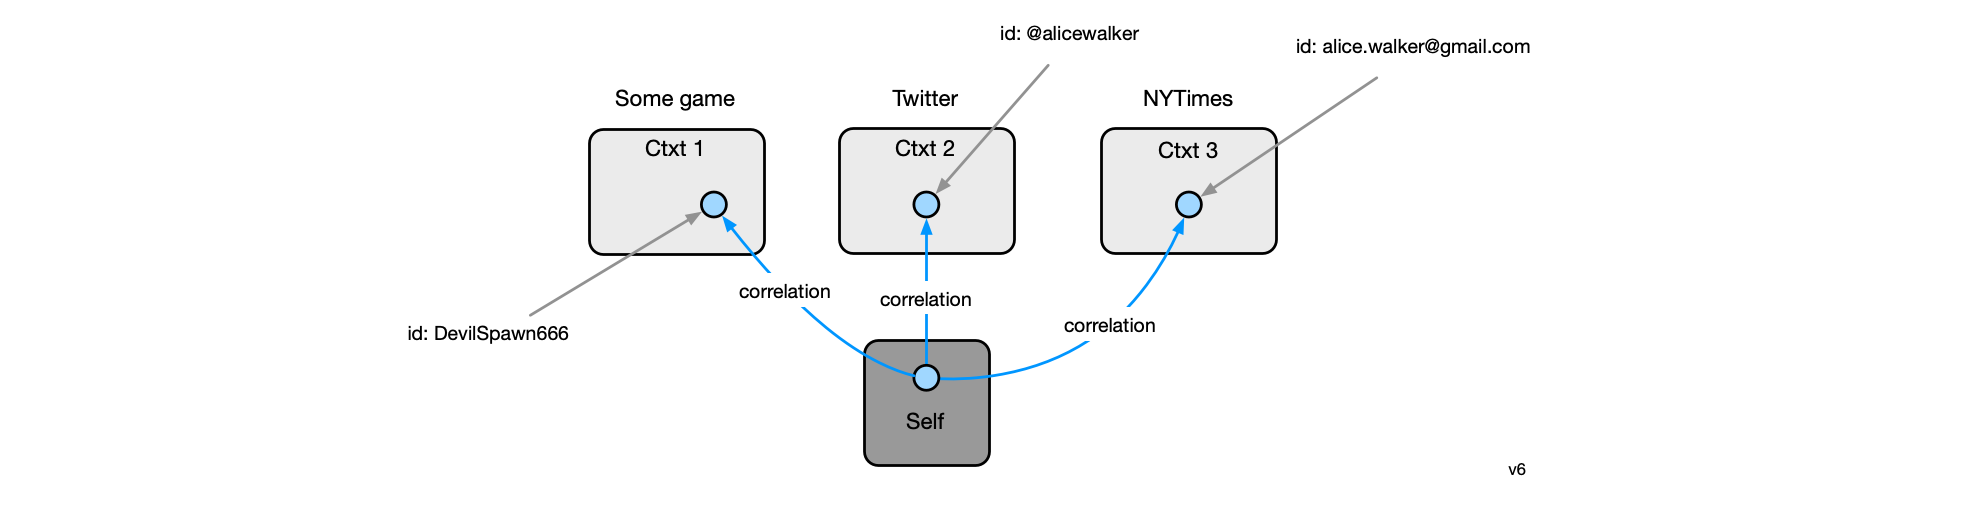
\includegraphics[width=\textwidth]{./images/example1.png}

\subsection{Functionality}

Here is a summary of the functionality of an example agent.

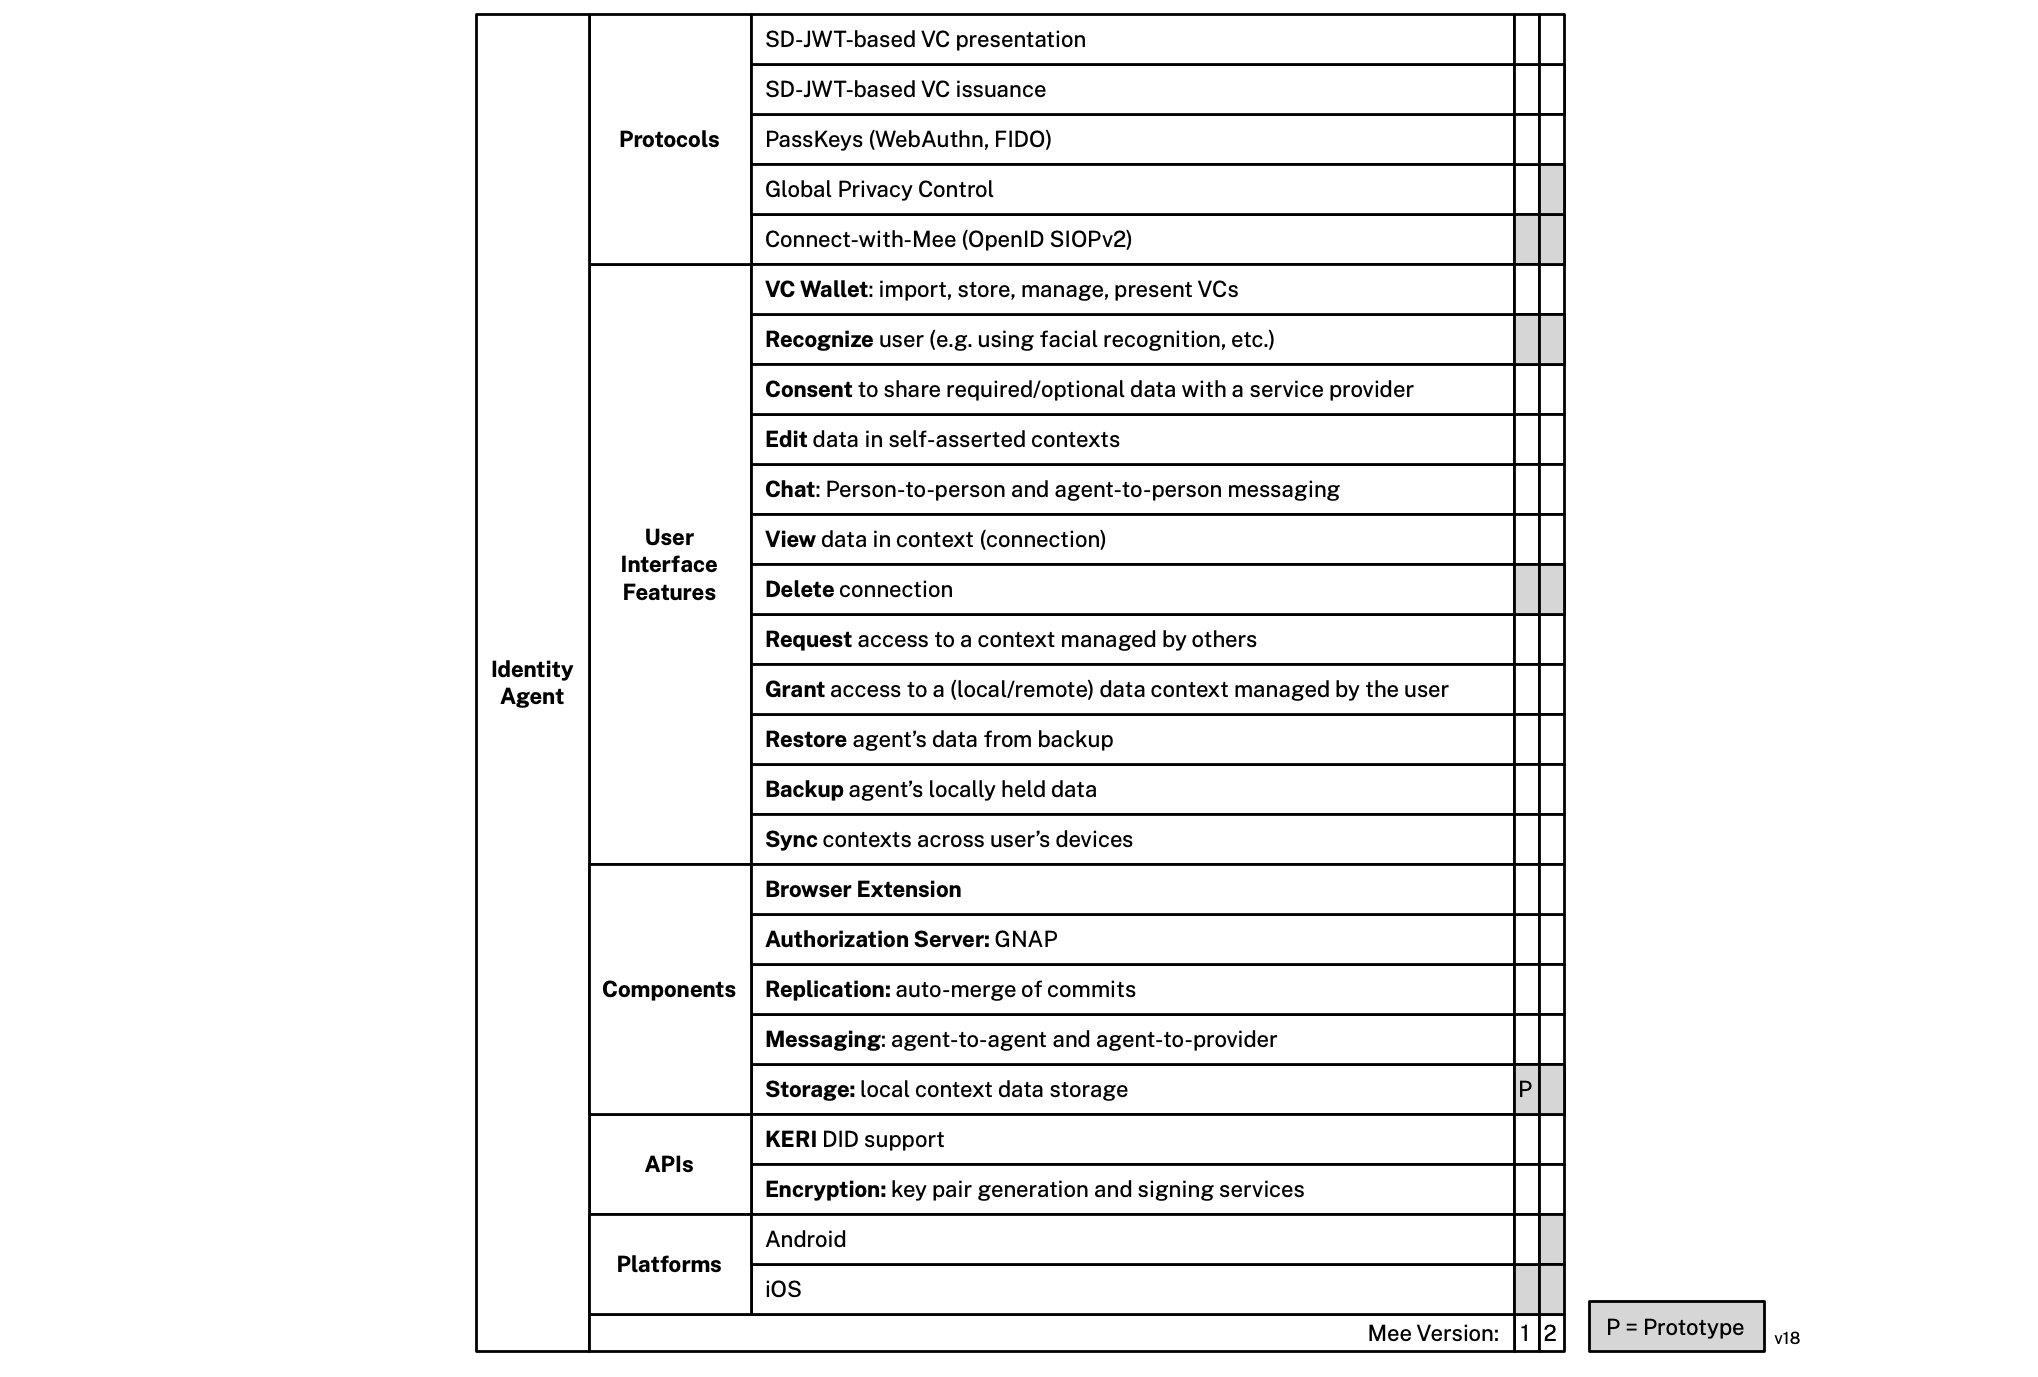
\includegraphics[width=\textwidth]{./images/agent-functionality.png}

\subsubsection{Protocols}

\begin{itemize}
\item SD JWT-based VC presentation
\item SD JWT-based VC issuance
\item PassKeys (WebAuthn)
\item Global Privacy Control
\item Connect-with-Mee: (OpenID SIOP) that uses a universal link to the agent
\end{itemize}

\subsubsection{UI Features}

\begin{itemize}
\item \textbf{VC Wallet:} import, store, manage, and present Verifiable Credentials (VCs). Note: the [OWF conceptual architecture](https://github.com/openwallet-foundation/architecture-task-force/blob/main/docs/architecture/conceptual-architecture.md) adds Burn, Receive, Send, Transfer, Refund, Purchase, Withdrawal, Deposit
\item \textbf{Recognize} user (e.g. using facial recognition, etc.)
\item \textbf{Consent} to share required/optional data with a service provider
\item \textbf{Edit} data in self-asserted contexts
\item \textbf{Chat:} Person-to-person and agent-to-person messaging
\item \textbf{View} data in contexts
\item \textbf{Delete connection} delete all data associated with this set of contexts
\item \textbf{Request} access to a context managed by others
\item \textbf{Grant} access to a (local or remote) data context managed by the user
\item  \textbf{Restore:} recover all data using SRP and backups
\item \textbf{Backup} local contexts
\item \textbf{Sync} contexts across user's devices
\end{itemize}

\subsubsection{Components}

\begin{itemize}
\item \textbf{Authorization Server}: GNAP AS
\item \textbf{Replication}: synchronization of context state across the user's set of agents
\item \textbf{Messaging}: communications among members of the user's set of agents
\item \textbf{Storage}: local data storage for contexts  
\end{itemize}

\subsection{Architecture}

In this section we propose an architecture for identity agents. We consider a user, Alice, and her agent's three layered architecture shown below.

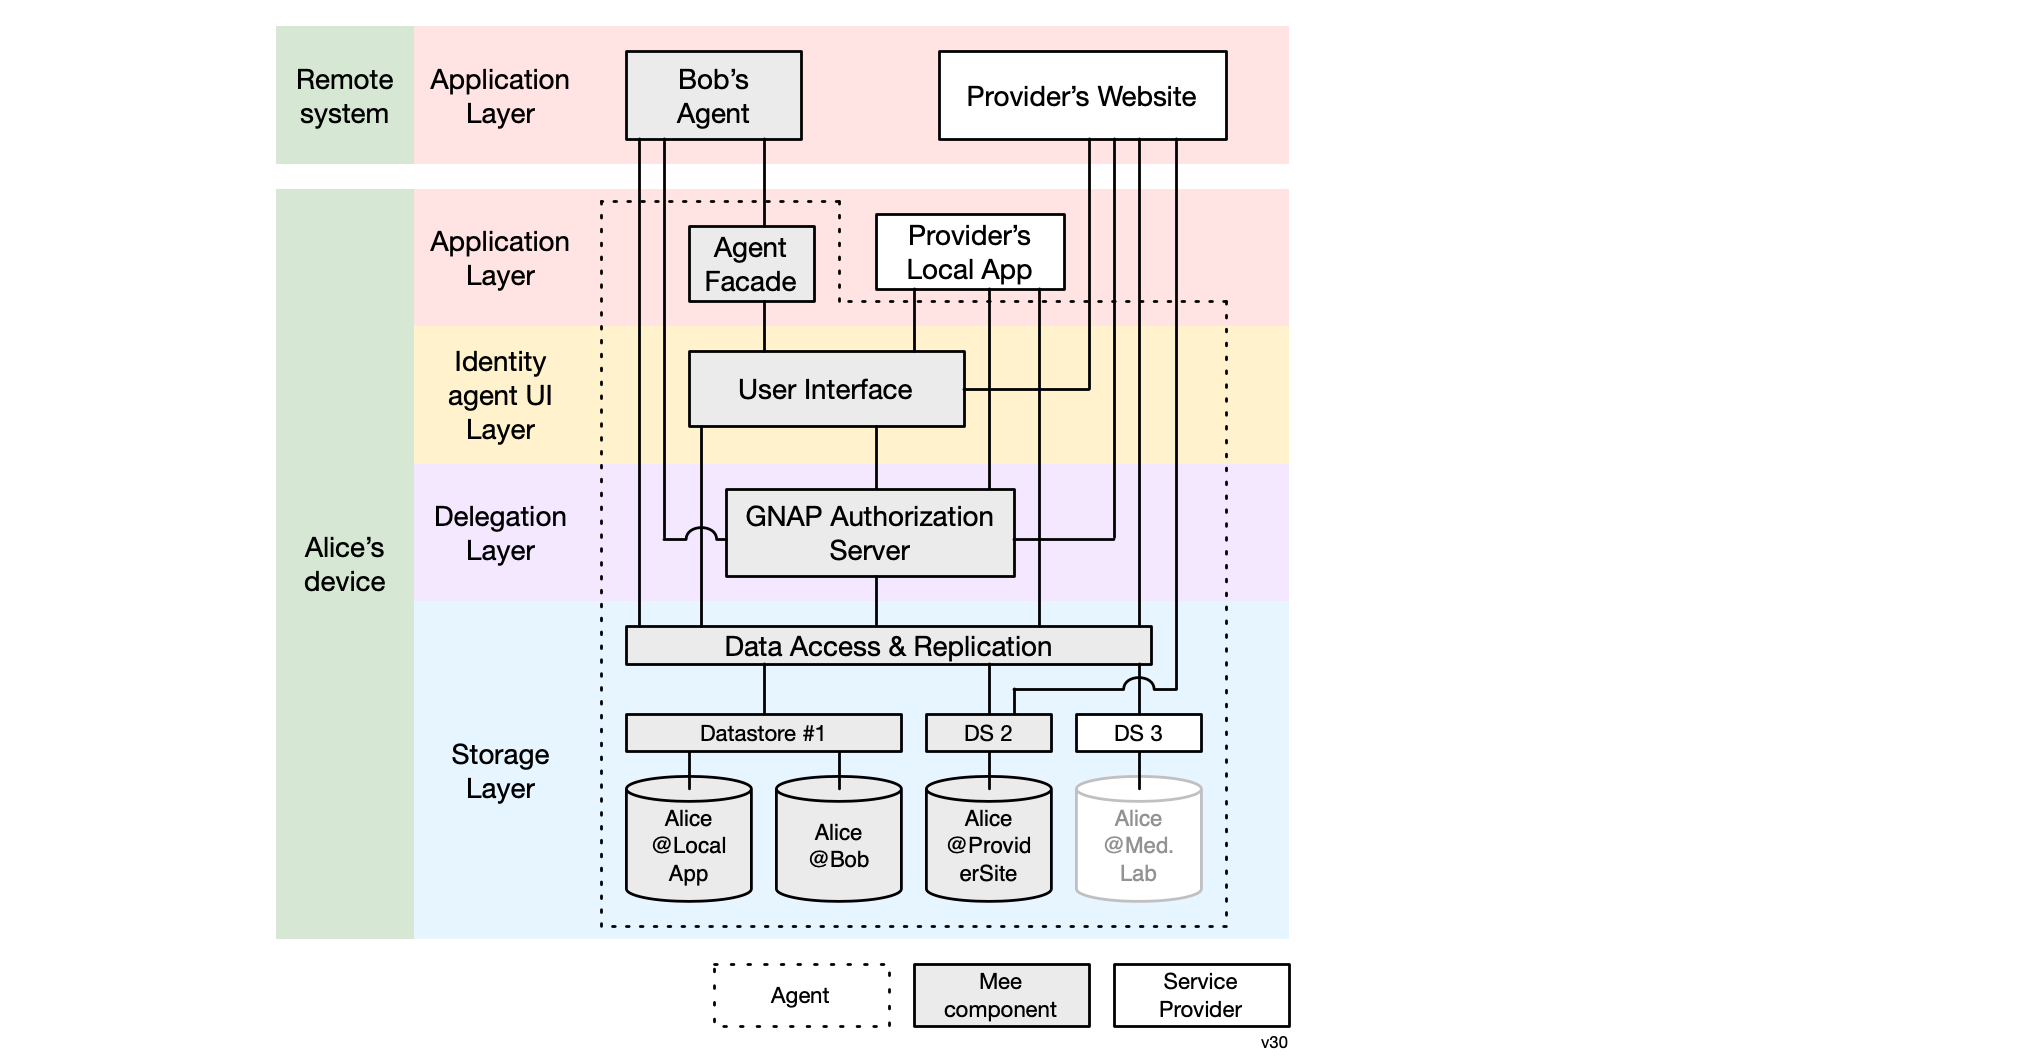
\includegraphics[width=\textwidth]{./images/architecture.png}

\subsubsection{UI layer}

Alice's identity agent is deployed as an app on Alice's device (e.g. a smart phone). The top, UI layer provides Alice with data management features to connect with apps/sites and manage her data. This UI allows her to inspect and in some cases edit each of the partial representations of her in each connection's context(s). Part of this UI is an "agent facade"--a presentation layer for how Alice appears to other agent users. 

\subsubsection{Delegation layer}

The \hyperfootnote[GNAP][https://]{oauth.net/gnap/} Authorization Server (AS) responds to requests for access to Alice's context datastores wherever they may be located physically. These requests could come from any app/site whether local or remote. In other words they could come from local apps (e.g. Provider's App), remote app/sites (e.g. Provider's Website) or from other users' agents (e.g. Bob's Agent). The AS is integrated with the agent's UI to allow Alice to grant or deny these requests for access. If Alice, either through explicit UI interaction or via a policy she has established, grants the request, the AS returns an access token to the requester. The requester presents this access token to a context datastore when it needs access. 

\subsubsection{Storage layer}

The Data Access and Replication component has two responsibilities. First, it provides an abstraction layer performing schema mapping such that the UI layer with which it is integrated has read/write access to context data in an abstract, universal schema. This is the ``data access" responsibility. The second responsibility is to manage the replication of data within Alice's context datastores across all of Alice's devices (phone, tablet, laptop, etc.). 

Below the Data Access and Replication component lie a set of datastores each using its own datastorage technology to hold one or more contexts (data containers). Each context holds a contextualized representation of Alice as defined (as to schema) and created and managed by apps/sites. The diagram above shows three local contexts on Alice's device and one, the Med Lab app's context, which is not replicated on Alice's local device (perhaps because its data set is too large for Alice's device).

In this example, Bob's agent is accessing a context called ``Alice@Bob" as managed by datastore 1. Provider's Local App is accessing a context called ``Alice@Local App" that is also managed by datastore 1.  An external Provider's Website is accessing a context called ``Alice@ProviderSite" that is managed by datastore 2. 

\section{Applications}

We now consider how an identity agent interacts with applications. The diagram below shows Alice's agent from the previous section with the addition of a local as well as a remote application layer. 

\subsection{Interactions with apps/sites}

The local application layer contains applications that run on the same device as Alice's agent. The digram shows one such application labelled ``Provider's Local App". The remote application layer contains applications that run on systems and devices external to Alice's device. Two examples are shown. The first is Bob's Agent which appears to Alice as an app (just as Alice's agent appears as an app to Bob's agent). The second is a website labeled ``Provider's Website". 

The first step setting up a connection with a provider's app/site is for the app/site to authenticate the user's agent. We propose that the app/site implement the \hyperfootnote[OpenID SIOPv2][https://]{openid.net/specs/openid-connect-self-issued-v2-1\_0.html} for this purpose.

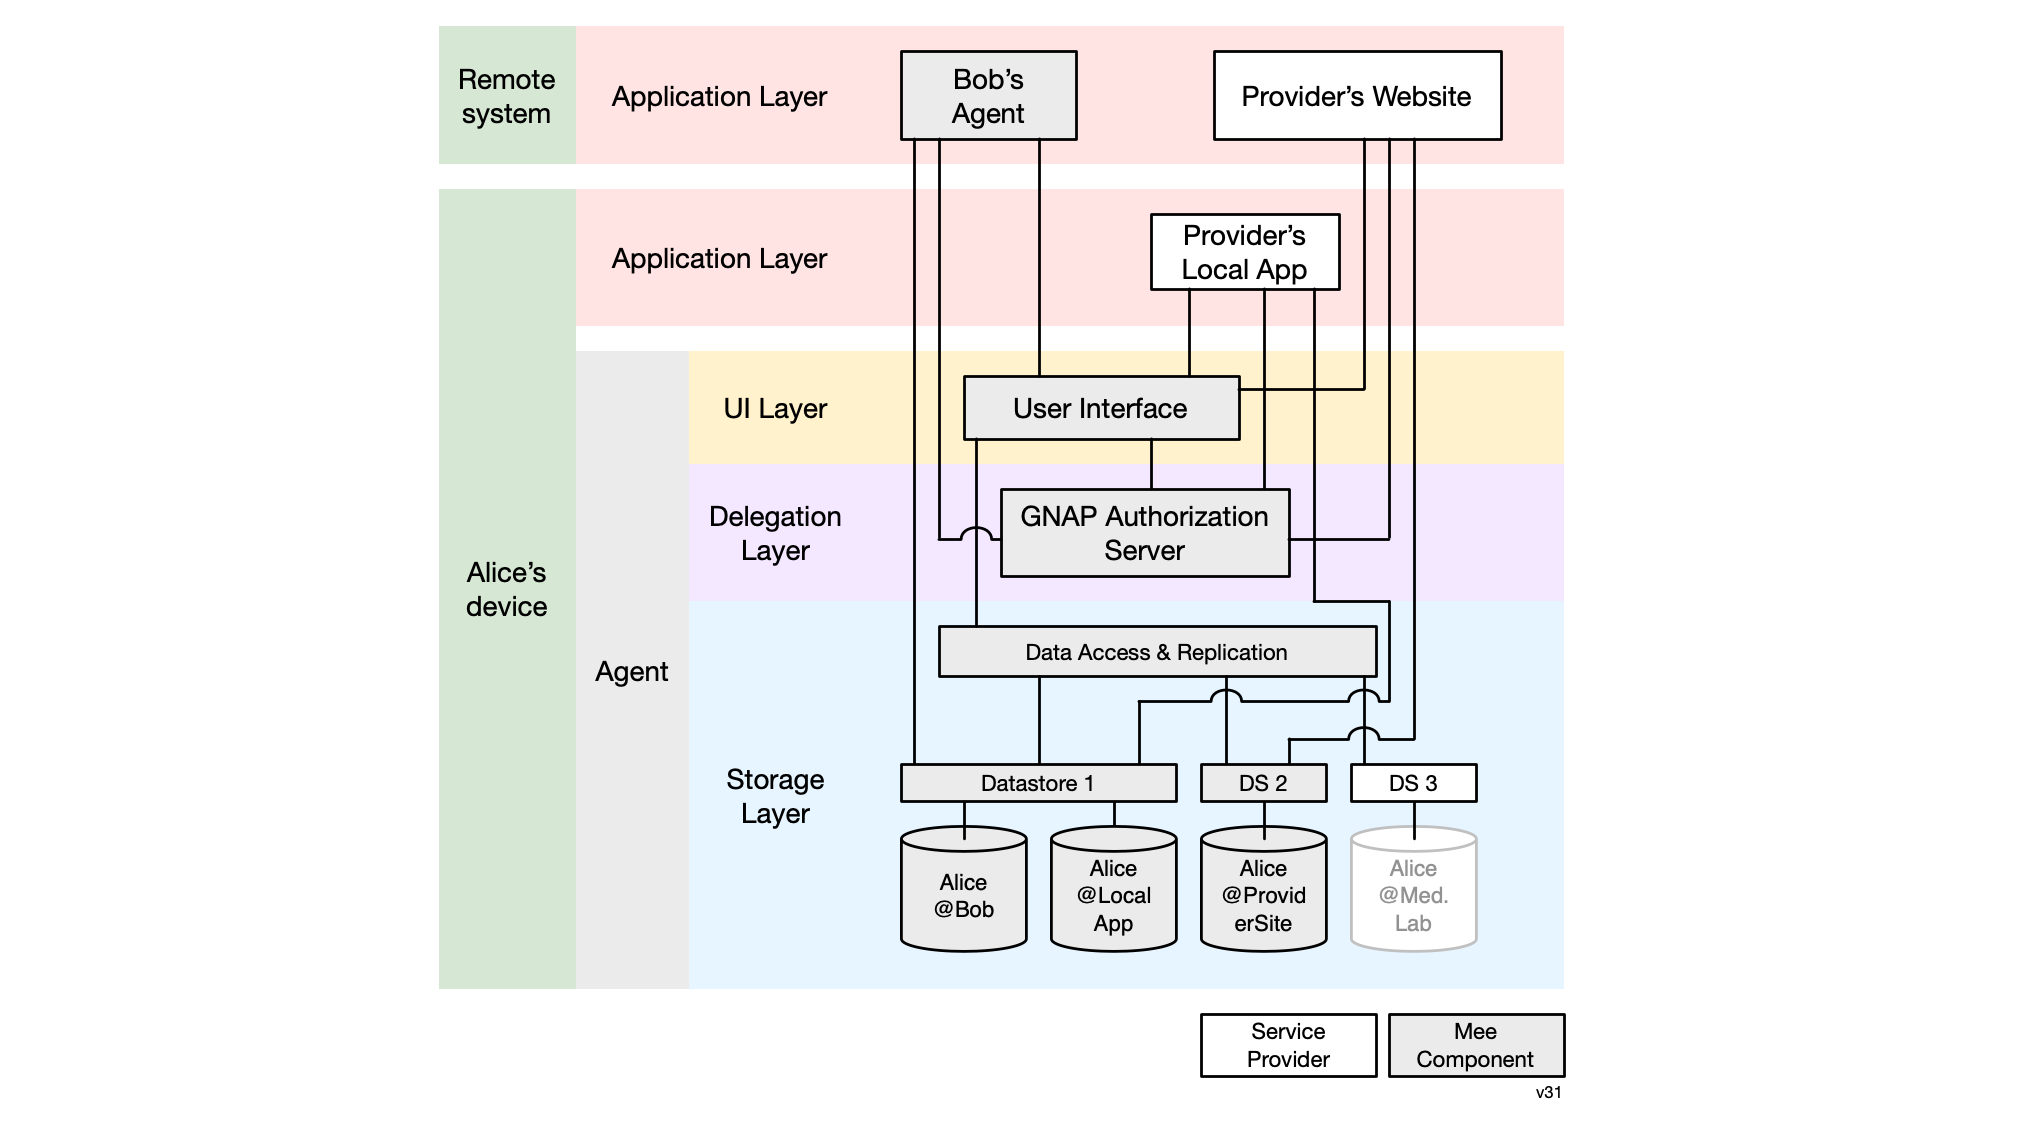
\includegraphics[width=\textwidth]{./images/applications.png}

\subsection{Private data sharing}
Data collected and held by the user's agent is clearly under the user's control. But data that they have shared with another party also needs to be under their control. We call this \emph{private data sharing}. Since no technical means exist to control data transferred to another party, legal means must be used instead. The legal mechanism we propose is a ``Human Information License" (HIL) contract between two parties. The first is the digital service provider legal entity behind a given app/site. The second is a legal entity, likely a nonprofit, that represents agent users. For more details see the ``Human Information License" section.

The HIL imposes a number of obligations of the provider. Among them is the provider's requirement to respect the user's \emph{data rights} to access, correction (editing), and deletion of the information collected and held by them. The user may have shared information manually (e.g. by filling in a form, or other kinds of interactions) or online from their agent. The HIL requires the provider to implement \emph{data rights} APIs/protocols that an agent can use to remotely control this collected data.

These data rights APIs/protocols are an are of active research.  
    
\section{Human Information License}
[to be written]

\section{Contributors}
Contributors to this document include Alexander Yuhimenko, Sergey Kucherenko, Kiril Khalitov.   

\bibliographystyle{plain}
\bibliography{library}


\end{document}  